% Chapter 6 (two-cause rewrite, 2026-11). Every result number is a generated macro or table cell.
% Old text: chapters_old/chapter6.tex (git tag thesis-pre-two-causes).
\chapter{Results and Discussion}
\label{ch:results}

This chapter reports the outcome of the analyses and the evaluation of the proposed method.
In the following, we first examine the two causes of forgetting: the drift of the
representation (Section~\ref{sec:c6-s1}) and the conflict on the background label
(Section~\ref{sec:c6-s2}). Then, we compare our method with the baselines on the six streams
(Section~\ref{sec:c6-s3}), assess the contribution of each component
(Section~\ref{sec:c6-s4}) and study the impact of its settings (Section~\ref{sec:c6-s5}).
After that, we examine its robustness (Section~\ref{sec:c6-s6}), its cost
(Section~\ref{sec:c6-s7}) and its behaviour beyond documents (Section~\ref{sec:c6-s8}).
Finally, we analyse its errors (Section~\ref{sec:c6-s9}) and discuss the findings
(Section~\ref{sec:c6-s10}). Unless stated, every number is the mean over three runs on
LayoutLMv3 under the protocol of Section~\ref{sec:e-protocol}.

\section{Cause 1: Representation Drift}
\label{sec:c6-s1}
% SOURCE: old ch6 38-507 condensed; paper App. E; E1 four-encoder grid; E3 drift under the methods
\todo{to be written}

% =============================================================================
\section{Cause 2: The Background-Label Conflict}
\label{sec:c6-s2}

In this section, we test the three hypotheses of Section~\ref{sec:m-hypotheses} on
CIL-CORD, and then on the two other class-incremental streams. Every run changes one
intervention against the run it is compared with. Unless stated, a memory is CoLaR with
$50$ documents per session. Table~\ref{tab:ladder} lists the hypotheses with the result of
each intervention; for each one, we report whether its prediction holds (\emph{supports}),
fails (\emph{refutes}) or holds in part (\emph{partly}).

\begin{table}[!htbp]
  \centering
  \caption[The series of hypotheses on CIL-CORD]{\textbf{The series of hypotheses} on
  CIL-CORD (mean $\pm$ s.d.; AF: mean, negative when old sessions improve later; bold: our
  method). $^{r}$Uses the ground-truth labels of the stored documents. $^{e}$ER trains
  every layer and keeps $\nErCilBuf$ raw documents.}
  \label{tab:ladder}
  % the generated table is set to \textwidth of the paper's full-width float: give it that width, then scale
  \resizebox{\textwidth}{!}{\begin{minipage}{21.6cm}\setlength{\textwidth}{21.6cm}\footnotesize\setlength{\tabcolsep}{3pt}% AUTO-GENERATED by scripts/rca/make_clean_tables.py -- do not edit.
\begin{tabular*}{\textwidth}{@{\extracolsep{\fill}}l c c c l@{}}
\toprule
Hypothesis (\emph{prediction if true}) and intervention & Full-label F1$\uparrow$ & AA$\uparrow$ & AF$\downarrow$ & Outcome \\
\midrule
Naive fine-tuning (reference) & $13.0{\pm}0.2$ & $18.3{\pm}0.5$ & $91.3$ &  \\
\midrule
\multicolumn{5}{@{}l@{}}{\textbf{H1.} Only drift: forgetting is just harder. \emph{If true: a memory that retains under domain shift retains here.}} \\
\quad whole-document memory (CoLaR), shared softmax & $30.7{\pm}1.5$ & $33.5{\pm}1.0$ & $10.2$ & refutes \\
\quad raw-document memory (ER), shared softmax$^{e}$ & $21.2{\pm}7.3$ & $24.0{\pm}3.4$ & $67.4$ & refutes \\
\midrule
\multicolumn{5}{@{}l@{}}{\textbf{H2.} The labels are the cause: stale in the memory, wrong on the current documents. \emph{If true: repairing the labels closes the gap within a shared softmax.}} \\
\quad older stored documents relabelled at each boundary$^{r}$ & $76.5{\pm}2.3$ & $63.6{\pm}1.9$ & $-29.9$ & partly \\
\quad every stored document relabelled before each session$^{r}$ & $92.1{\pm}1.3$ & $91.3{\pm}1.3$ & $1.1$ & supports \\
\quad the same tokens masked instead, no label added$^{r}$ & $89.7{\pm}1.2$ & $88.5{\pm}1.5$ & $-4.9$ & partly \\
\quad MiB-style loss: ``O'' may mean ``O or another session's class'' & $60.0{\pm}1.2$ & $72.1{\pm}1.9$ & $25.4$ & partly \\
\quad replay softmax sliced, stale ``O'' kept & $45.9{\pm}1.6$ & $48.8{\pm}8.2$ & $15.8$ & partly \\
\midrule
\multicolumn{5}{@{}l@{}}{\textbf{H3.} The shared background normalisation. \emph{If true: one background per session closes the gap without true labels, given a memory.}} \\
\quad \textbf{CoLaR memory, session-blocked readout (CoLaR-SBR)} & $89.1{\pm}2.0$ & $88.4{\pm}2.6$ & $4.2$ & supports \\
\quad session-blocked readout, no memory & $11.4{\pm}2.3$ & $21.6{\pm}2.2$ & $87.5$ & supports \\
\quad CoLaR memory, blocked readout with a constant background logit & $82.4{\pm}6.9$ & $80.2{\pm}8.1$ & $0.2$ & partly \\
\quad ICE-O (our re-implementation): frozen encoder, constant Other logit, no memory & $57.0{\pm}0.7$ & $35.2{\pm}0.7$ & $0.0$ & partly \\
\midrule
Joint training (reference) & $93.1{\pm}1.0$ & $92.6{\pm}0.9$ & -- &  \\
\bottomrule
\end{tabular*}
\end{minipage}}
\end{table}

\subsection{H1: Only Harder Forgetting}
\label{sec:r-h1}

We first hypothesized that label growth only makes forgetting harder, i.e., that the
failure is still caused by drift. If so, a memory that works under domain shift should also
work here. However, the results refute it.

\paragraph{The same memory on the two settings.} On DIL, the CoLaR memory comes within
$\nColarDilGapMax$ AA points of joint training (Section~\ref{sec:c6-s3}). On CIL-CORD, the
same memory with a shared softmax reaches only $\vColarFull$ full-label F1 against
$\vJointFull$ for joint training. Raw documents do no better: ER with $\nErCilBuf$
documents reaches $\vErFull$. A larger memory does not close the gap either
(Section~\ref{sec:c6-s5}). Hence, what removes the drift on a fixed label space does not
remove the failure under label growth.

\paragraph{The diagonal of the retention matrix.} Besides, the failure does not look like
ordinary forgetting (Figure~\ref{fig:heatmaps}). Naive fine-tuning forgets the old sessions
but learns each new session well, to at least $\nNaiveDiagMin$ F1 right after it is
trained. In contrast, with the memory the model fails to learn the session that it is
training on: from session~3 on, the diagonal of CoLaR is low, and its newest session ends
at only $\mColarLastMin$ to $\mColarLastMax$ F1. It is noted that this is not due to the
frozen layers, since our readout learns every session to at least $\nSbrDiagMin$ F1 with
the same frozen layers and the same memory. The memory does keep a part of the past: the
model retains $\mColarRMin$ to $\mColarRMax\%$ of the entities of the old sessions, where
naive fine-tuning keeps none. Therefore, the replayed documents help the old classes and
work against the new ones, which is the stored side of the conflict of
Section~\ref{sec:m-conflict-origin}.

\paragraph{Outcome.} Drift alone does not explain the failure, and H1 is refuted.

\begin{figure}[!htbp]
  \centering
  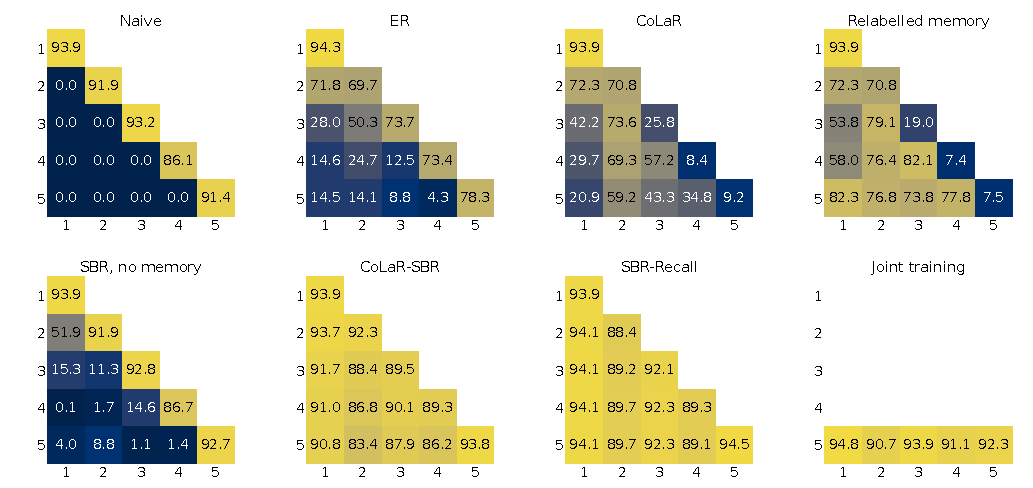
\includegraphics[width=\textwidth]{paper/heatmaps.pdf}
  \caption[Retention matrices on CIL-CORD]{\textbf{Retention matrices} on CIL-CORD
  (session-restricted F1). Row $i$: after training session $i$; column $j$: session $j$.
  Joint training is one pooled run, so only its final row exists.}
  \label{fig:heatmaps}
\end{figure}

\subsection{H2: The Labels Are the Cause}
\label{sec:r-h2}

We next hypothesized that the labels are the cause, on the stored side and on the current
side. If so, repairing the labels should close the gap with the shared softmax unchanged.

\paragraph{Stored side.} We repair the stored labels with the ground-truth labels, which a
continual learner does not have. When every stored document is relabelled \emph{before
each session} with the true labels of all classes in the grown head, the same memory and
the same softmax reach $\vOraclePreFull$ full-label F1, within $\nOraclePreJointGap$ points
of joint training. Masking the stale tokens in the replay loss, which removes the false
background label without adding a label, reaches $\vOracleMaskFull$. Hence, removing the
stale negatives alone recovers most of the gap on this stream. The timing of the repair
matters. When the older stored documents are relabelled only at the session boundaries,
the documents of the session that is being trained are not yet covered, and the repair
helps one session too late: \gls{aa} rises from $\nColarSeed$ to $\nOracle$, but
sessions~3 to~5 are learned only to $\nOracleLateMin$ to $\nOracleLateMax$ F1 on their own
diagonal, sessions~3 and~4 rise to $\nOracleNextMin$ to $\nOracleNextMax$ one session
later, and the last session ends at $\nOracleLast$.

\paragraph{Current side.} We then repair the loss, which needs no additional annotation.
The MiB-style loss of Equation~\eqref{eq:mib} lifts the full-label F1 to $\vMibFull$, i.e.,
$\nMibShareFull\%$ of the gap to joint training. It learns every session to at least
$\nMibDiagMin$ F1; however, the first session ends at no more than $\nMibFirstMax$ F1 in
any run. Slicing the softmax of the replay loss reaches only $\vSlicedFull$, and slicing
both losses, the control inspired by SS-IL, reaches $\vSlicedBothFull$. It is noted that
the sliced variant trains unstably: within a session, its validation F1 can collapse after
its peak. Thus, a repair of the loss helps only partly on CIL-CORD. Besides, the
ground-truth labels above close the gap although every current document still labels old
entities as background; hence, the current side does not prevent this rescue on CIL-CORD.

\paragraph{The other streams.} The picture changes with the stream
(Figure~\ref{fig:repairs}, Table~\ref{tab:repairs}). On CIL-FUNSD, the ground-truth stored
labels leave the shared softmax where it was, whereas the MiB-style loss is level with our
readout. On CIL-WildReceipt, the ground-truth labels help only partly, and the MiB-style
loss stays below our readout. This can be due to the share of the two sides in each stream:
in CIL-FUNSD, the forms of the second session contain the questions of the first one, so
the current side dominates, whereas in CIL-CORD the stored documents carry many stale
labels.

\paragraph{Outcome.} H2 is only partly supported: repairing the labels helps, but no label
repair closes the gap on every stream.

\begin{figure}[!htbp]
  \centering
  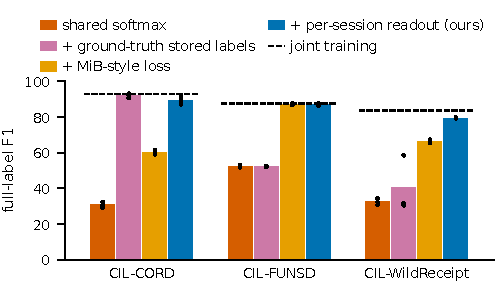
\includegraphics[width=0.62\textwidth]{paper/repairs.pdf}
  \caption[Three repairs on three class-incremental streams]{\textbf{Three repairs on three
  class-incremental streams} (full-label F1; dashed: joint training). Only the per-session
  readout closes most of the gap on all three streams.}
  \label{fig:repairs}
\end{figure}

\begin{table}[!htbp]
  \centering
  \caption[Three repairs on three class-incremental streams: values]{\textbf{Three repairs
  on three class-incremental streams} (full-label F1, mean $\pm$ s.d.). Every row but the
  last uses the same CoLaR memory, and the first three keep the shared softmax. The
  ground-truth stored labels are not available to a continual learner.}
  \label{tab:repairs}
  % AUTO-GENERATED by scripts/rca/make_clean_tables.py -- do not edit.
\begin{tabular}{lccc}
\toprule
Repair & CIL-CORD & CIL-FUNSD & CIL-WildReceipt \\
\midrule
Shared softmax (CoLaR) & $30.7{\pm}1.5$ & $52.2{\pm}0.6$ & $32.5{\pm}1.8$ \\
+ ground-truth stored labels & $92.1{\pm}1.3$ & $52.2{\pm}0.2$ & $40.3{\pm}15.9$ \\
+ MiB-style loss & $60.0{\pm}1.2$ & $87.3{\pm}0.4$ & $66.5{\pm}0.8$ \\
+ per-session readout (CoLaR-SBR) & $89.1{\pm}2.0$ & $87.2{\pm}0.6$ & $79.5{\pm}0.3$ \\
\midrule
Joint training (reference) & $93.1{\pm}1.0$ & $87.5{\pm}0.8$ & $83.7{\pm}1.0$ \\
\bottomrule
\end{tabular}

\end{table}

\subsection{H3: The Shared Normalisation}
\label{sec:r-h3}

Finally, we hypothesized that the conflict lives in the shared normalisation: one
background logit trained by documents that disagree on the background. If so, one
background logit per session, normalised with the tags of that session only, should close
most of the gap without additional annotations.

\paragraph{With the memory.} The hypothesis is supported. With the memory, the blocked
readout (CoLaR-SBR) reaches $\vSbrFull$ full-label F1, $\nSbrGapFullMin$ to
$\nSbrGapFullMax$ points below joint training, and no ground-truth label is used. Every
session is learned when it is trained, and the columns of its retention matrix hold
(Figure~\ref{fig:heatmaps}). Regarding the remaining gap, a session loses $\sbrLossMin$ to
$\sbrLossMax$ points from its diagonal to the final row, session~$\sbrLossMaxSession$ the
most. Hence, what CoLaR-SBR still loses to joint training is the retention of the early
sessions.

\paragraph{Without the memory.} Without the memory, the same readout scores only
$\vNoBankFull$. The reason is not the conflict: no old entity token is predicted as ``O''.
Instead, $\mNoBankOtherMin$ to $\mNoBankOtherMax\%$ of the wrong tokens receive a class of
another session, and each old block claims $\mNoBankFalseMin$ to $\mNoBankFalseMax\%$ of
the tokens of its own test split that are not its entities, against $\mSbrFalseMin$ to
$\mSbrFalseMax\%$ with the memory. This is consistent with an encoder that has drifted
under a readout that no longer fits it. Thus, the readout removes the conflict and the
memory removes the drift; neither replaces the other (Section~\ref{sec:c6-s4}).

\paragraph{Where the entities of old sessions go.} Figure~\ref{fig:findings} summarises
the three hypotheses and shows, for the final model, where the entities of the old sessions
end. Under CoLaR-SBR, the owning block claims $\mSbrOwnerMin$ to $\mSbrOwnerMax\%$ of the
old entity tokens, and most of the remaining errors ($\mSbrSameMin$ to $\mSbrSameMax\%$ of
the wrong tokens) give the token another tag of its own session. Therefore, the blocks
rarely confuse the sessions; what is left is the usual confusion between the classes of
one session. With a shared softmax and a memory, the newest session is suppressed, whereas
naive fine-tuning learns it and keeps nothing older (Figure~\ref{fig:findings}c).

\paragraph{Outcome.} H3 is supported on all three class-incremental streams
(Figure~\ref{fig:repairs}): the label-side repairs each succeed on one stream, whereas the
blocked readout closes most of the gap on all three. This motivates the readout of our
method.

\begin{figure}[!htbp]
  \centering
  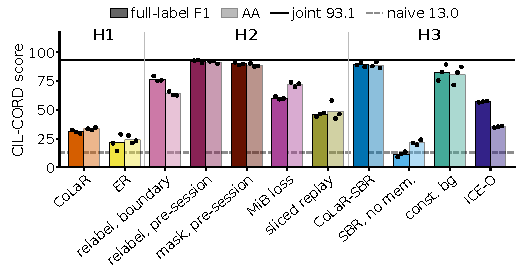
\includegraphics[width=0.56\textwidth]{paper/findings_a.pdf}\hfill
  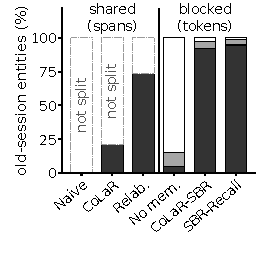
\includegraphics[width=0.21\textwidth]{paper/findings_b.pdf}\hfill
  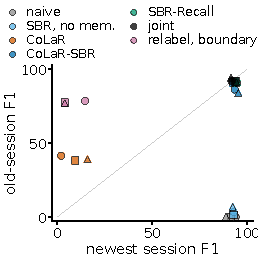
\includegraphics[width=0.21\textwidth]{paper/findings_c.pdf}\\
  \makebox[0.56\textwidth]{\small(a)}\hfill\makebox[0.21\textwidth]{\small(b)}\hfill\makebox[0.21\textwidth]{\small(c)}\\[2pt]
  
\includegraphics[width=0.6\textwidth]{paper/findings_b_key.pdf}
  \caption[The findings on CIL-CORD in one figure]{\textbf{The findings in one figure}
  (CIL-CORD). (a) The series of hypotheses: full-label F1 (dark) and AA (light). (b) Where
  the final model puts the entities of the old sessions. (c) F1 of the newest session
  against the mean F1 of the old sessions, one marker per run.}
  \label{fig:findings}
\end{figure}

\subsection{One Principle behind the Repairs}
\label{sec:r-principle}

The repairs of this section differ in what they change, but they follow one principle: a
stored background label must not count against a class that its document could not
annotate (Table~\ref{tab:scope}). The shared softmax violates it, the slices and the
MiB-style loss weaken the violation, the ground-truth labels remove it with information
that a continual learner does not have, and the per-session readout removes it in the
normalisation. As the results demonstrate, the three repairs that follow the principle fully
(the last three rows) come close to joint training, and the per-session readout is the
only one of them that needs no ground-truth label.

\begin{table}[!htbp]
  \centering
  \caption[One principle, six repairs]{\textbf{One principle, six repairs} (CIL-CORD, same
  CoLaR memory, full-label F1): how each repair treats a stored background label.
  $^{r}$Uses the ground-truth labels.}
  \label{tab:scope}
  \begin{tabular}{@{}llc@{}}
    \toprule
    Repair & Treatment of a stored background label & F1 \\
    \midrule
    Shared softmax & background against all entities & $\vColarFull$ \\
    Softmax slice & background against the entities known at storage & $\vSlicedFull$ \\
    MiB-style loss & marginal target: ``O or a later class'' & $\vMibFull$ \\
    Stale tokens masked$^{r}$ & no loss where the label is stale & $\vOracleMaskFull$ \\
    True stored labels$^{r}$ & corrected to the true label & $\vOraclePreFull$ \\
    Per-session readout (SBR) & background within its own session & $\vSbrFull$ \\
    \bottomrule
  \end{tabular}
\end{table}

% =============================================================================
\section{Main Comparison on Six Streams}
\label{sec:c6-s3}

The results on the six streams are shown in Table~\ref{tab:main}. Overall, naive
fine-tuning forgets heavily on every stream but DIL-XFUND, and no baseline with a shared
softmax comes close to joint training on the class-incremental streams. In contrast,
CoLaR-SBR or its memory-free variant achieves the best result on the three
class-incremental streams and on Mixed.

\begin{landscape}
\begin{table}[p]
  \centering
  \caption[Comparison with the baselines on six streams]{\textbf{Comparison with
  continual-learning baselines} on six streams. F1: full-label F1; AA and AF: average
  accuracy and forgetting. AA and F1: mean $\pm$ s.d.; AF: mean; ``--'': not applicable.
  Bold: best AA and F1 of each column, joint training aside; underlined: our best when a
  baseline is best. $^{b}$With the $50$-document memory.}
  \label{tab:main}
  \resizebox{\linewidth}{!}{% AUTO-GENERATED by scripts/rca/make_clean_tables.py -- do not edit.
\begin{tabular}{@{}llccccccccccccc@{}}
\toprule
 & & \multicolumn{3}{c}{CIL-CORD} & \multicolumn{2}{c}{Mixed} & \multicolumn{2}{c}{DIL} & \multicolumn{2}{c}{CIL-FUNSD} & \multicolumn{2}{c}{CIL-WildReceipt} & \multicolumn{2}{c}{DIL-XFUND} \\
\cmidrule(lr){3-5}\cmidrule(lr){6-7}\cmidrule(lr){8-9}\cmidrule(lr){10-11}\cmidrule(lr){12-13}\cmidrule(l){14-15}
Family & Method & F1$\uparrow$ & AA$\uparrow$ & AF$\downarrow$ & AA$\uparrow$ & AF$\downarrow$ & AA$\uparrow$ & AF$\downarrow$ & AA$\uparrow$ & AF$\downarrow$ & AA$\uparrow$ & AF$\downarrow$ & AA$\uparrow$ & AF$\downarrow$ \\
\midrule
Reference & Naive fine-tuning & $13.0{\pm}0.2$ & $18.3{\pm}0.5$ & $91.3$ & $42.1{\pm}0.7$ & $54.6$ & $39.2{\pm}0.3$ & $71.7$ & $43.9{\pm}0.5$ & $86.1$ & $19.6{\pm}0.1$ & $82.7$ & $71.2{\pm}0.7$ & $7.5$ \\
 & Joint training & $93.1{\pm}1.0$ & $92.6{\pm}0.9$ & -- & $87.6{\pm}0.7$ & -- & $86.7{\pm}0.2$ & -- & $87.9{\pm}0.7$ & -- & $83.5{\pm}0.8$ & -- & $79.5{\pm}0.4$ & -- \\
\midrule
Regularisation & LwF (2016) & $13.0{\pm}0.4$ & $18.5{\pm}0.6$ & $90.5$ & $44.2{\pm}1.4$ & $52.8$ & $37.6{\pm}1.1$ & $73.7$ & $44.0{\pm}0.3$ & $84.4$ & $19.8{\pm}0.3$ & $82.5$ & $72.0{\pm}0.2$ & $4.8$ \\
\midrule
Replay & ER (2019) & $21.2{\pm}7.3$ & $24.0{\pm}3.4$ & $67.4$ & $76.4{\pm}3.3$ & $6.9$ & $87.0{\pm}0.2$ & $0.1$ & $47.4{\pm}3.9$ & $72.0$ & $20.3{\pm}0.4$ & $77.7$ & $79.3{\pm}1.0$ & $-2.4$ \\
 & DER++ (2020) & $18.6{\pm}6.4$ & $21.2{\pm}1.6$ & $82.5$ & $73.7{\pm}4.6$ & $18.1$ & $\mathbf{88.2{\pm}1.8}$ & $2.5$ & $46.6{\pm}6.2$ & $75.2$ & $19.7{\pm}0.7$ & $81.3$ & $\mathbf{80.2{\pm}0.3}$ & $-1.0$ \\
\midrule
Prompt, LoRA & CODA-Prompt (2023) & $5.6{\pm}3.8$ & $7.3{\pm}4.7$ & $28.6$ & $8.5{\pm}0.8$ & $33.7$ & $31.0{\pm}0.2$ & $35.4$ & $10.0{\pm}6.5$ & $17.3$ & $14.0{\pm}0.1$ & $68.3$ & $30.9{\pm}0.3$ & $-3.7$ \\
 & CL-LoRA (2025) & $12.8{\pm}0.6$ & $18.4{\pm}0.6$ & $73.8$ & $41.3{\pm}0.4$ & $51.1$ & $42.5{\pm}0.8$ & $60.6$ & $41.2{\pm}1.2$ & $79.0$ & $18.2{\pm}0.4$ & $78.0$ & $53.6{\pm}5.2$ & $9.3$ \\
\midrule
Continual NER & CPFD (2023) & $4.5{\pm}6.7$ & $6.3{\pm}10.6$ & $30.2$ & $2.0{\pm}3.5$ & $38.7$ & $0.0{\pm}0.0$ & $56.2$ & $23.3{\pm}21.1$ & $79.6$ & $7.8{\pm}9.9$ & $26.7$ & $1.8{\pm}3.2$ & $39.9$ \\
 & IS3 (2024) & $8.7{\pm}1.2$ & $5.2{\pm}1.5$ & $43.8$ & $14.0{\pm}24.3$ & $39.6$ & $38.4{\pm}0.3$ & $37.4$ & $27.0{\pm}0.2$ & $83.9$ & $4.1{\pm}0.1$ & $39.0$ & $64.7{\pm}1.4$ & $8.0$ \\
\midrule
Merging & LCA (2026) & $10.9{\pm}0.7$ & $8.8{\pm}1.2$ & $56.4$ & $33.9{\pm}7.1$ & $26.9$ & $41.1{\pm}2.6$ & $30.2$ & $56.6{\pm}4.3$ & $35.4$ & $32.1{\pm}7.5$ & $40.3$ & $65.1{\pm}1.3$ & $-0.3$ \\
\midrule
\rowcolor{black!7}Ours & CoLaR (memory only) & $30.7{\pm}1.5$ & $33.5{\pm}1.0$ & $10.2$ & $74.7{\pm}6.8$ & $11.3$ & $\underline{86.5{\pm}0.7}$ & $0.7$ & $45.0{\pm}0.2$ & $85.8$ & $22.8{\pm}4.8$ & $57.5$ & $\underline{76.9{\pm}1.6}$ & $-1.9$ \\
\rowcolor{black!7} & CoLaR-SBR & $89.1{\pm}2.0$ & $88.4{\pm}2.6$ & $4.2$ & $\mathbf{89.1{\pm}0.6}$ & $-0.1$ & $85.4{\pm}0.4$ & $3.7$ & $87.4{\pm}0.6$ & $-1.4$ & $79.4{\pm}0.3$ & $1.6$ & $76.4{\pm}0.5$ & $-2.4$ \\
\rowcolor{black!7} & SBR-Recall & $\mathbf{92.6{\pm}1.0}$ & $\mathbf{91.9{\pm}0.6}$ & $-0.4$ & $84.8{\pm}1.0^{b}$ & $3.5$ & $31.8{\pm}1.7$ & $37.4$ & $\mathbf{87.6{\pm}1.7}$ & $0.1$ & $\mathbf{81.1{\pm}0.4}$ & $-0.2$ & $52.1{\pm}3.5$ & $8.6$ \\
\bottomrule
\end{tabular}
}
\end{table}
\end{landscape}

\paragraph{Results on the class-incremental streams.} On CIL-CORD, CoLaR-SBR achieves
$\vSbrFull$ full-label F1 ($\vSbr$ AA), which significantly improves over the same memory
with a shared softmax ($\vColarFull$) and comes close to the upper-bound baseline, joint
training ($\vJointFull$). Our method also surpasses the other baselines by a large margin:
the best of them, ER with $\nErCilBuf$ raw documents, reaches only $\vErFull$.
Interestingly, the continual NER methods CPFD and IS3, which are designed for the shift of
the background label, do not benefit either; this can be due to the shared softmax that
they keep. On top of that, SBR-Recall gains the highest
score ($\vRecallFull$) with no stored document. We observe the same pattern on the two
other class-incremental streams. On CIL-FUNSD, CoLaR-SBR reaches $\vFunsdSbr$ AA, level
with joint training ($\vFunsdJoint$), whereas CoLaR with a shared softmax stays close to
naive fine-tuning ($\vFunsdColar$ against $\vFunsdNaive$). On CIL-WildReceipt, CoLaR-SBR
reaches $\vWildSbr$ AA against $\vWildColar$ for the shared softmax; nevertheless, our
method still has a gap to joint training there ($\vWildJoint$).

\paragraph{Results on the domain-incremental streams.} On a fixed label space there is one
block and nothing to separate; hence, these streams test the memory alone. On DIL, naive
fine-tuning reaches only $\vNaiveDil$ AA against $\vJointDil$ for joint training, whereas
every replay method comes close to joint training (ER: $\vErDil$, CoLaR: $\vColarDil$,
CoLaR-SBR: $\vSbrDil$). Thus, it is reasonable that the blocked readout brings no gain
here. On DIL-XFUND, where only the language changes, forgetting is milder ($\vXfundNaive$
for naive fine-tuning against $\vXfundJoint$ for joint training). CoLaR and CoLaR-SBR
improve over naive fine-tuning ($\vXfundColar$ and $\vXfundSbr$), but they stay below ER
and DER++ ($\vXfundEr$ and $\vXfundDerPp$), which keep raw documents and train every
layer. This hints that the frozen lower layers limit the adaptation to a new language, in
particular to a new script. As predicted in Section~\ref{sec:m-recall}, SBR-Recall, which
has no memory and nothing to select its states by on a fixed label space, falls below
naive fine-tuning on both streams ($\vRecallDil$ on DIL).

\paragraph{Results on the Mixed stream.} On Mixed, the sessions change the classes, the
domain and the annotation schema. Naive fine-tuning reaches $\vNaiveMix$ AA. A memory
under a shared softmax helps (ER: $\vErMix$, CoLaR: $\vColarMix$), but it leaves a gap to
joint training ($\vJointMix$). In contrast, CoLaR-SBR gains the highest \gls{aa} among all
methods ($\vSbrMix$), on par with joint training and with almost no forgetting. SBR-Recall
needs the memory on this stream: it reaches $\nRecallMixMem$ AA with the $50$-document
memory and only $\nRecallMixNoMem$ without it.

\paragraph{Forgetting analysis.} Figure~\ref{fig:forgetting} follows the F1 over the
sessions of CIL-CORD. After the five sessions, naive fine-tuning keeps $\nFirstNaive$ F1
on session~1 and CoLaR with a shared softmax $\nFirstColar$, whereas CoLaR-SBR keeps
$\nFirstSbr$ and SBR-Recall $\nFirstRecall$. CoLaR-SBR and SBR-Recall stay close to joint
training after every session, whereas the methods with a shared softmax lose session~1
step by step. It is noted that CoLaR with a shared softmax has a low \gls{af} only because
it suppresses each new session while learning it; hence, \gls{af} must be read together
with \gls{aa} and with the diagonal of the retention matrix.

\begin{figure}[!htbp]
  \centering
  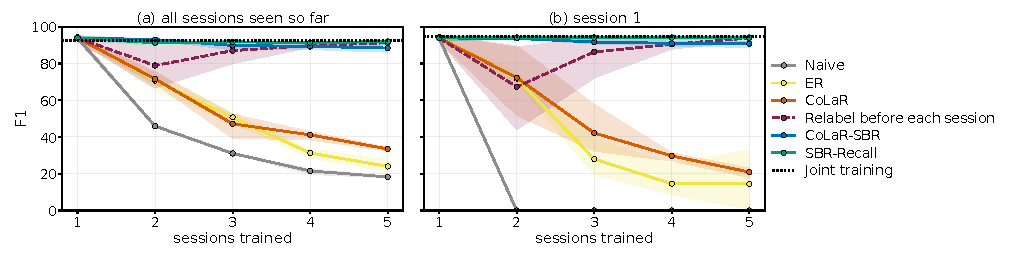
\includegraphics[width=\textwidth]{paper/forgetting.pdf}
  \caption[Forgetting on CIL-CORD]{\textbf{Forgetting on CIL-CORD}, session by session
  (line: mean of three runs, band: their range). (a) F1 averaged over the sessions seen so
  far. (b) F1 of session~1.}
  \label{fig:forgetting}
\end{figure}

% =============================================================================
\section{Component Ablation}
\label{sec:c6-s4}

To assess the contribution of each component of CoLaR-SBR, we conduct an ablation study on
CIL-CORD (Table~\ref{tab:components}). Starting from naive fine-tuning (Index~I), we add
the CoLaR memory, the session-blocked readout and the learned background logit.

\begin{table}[!htbp]
  \centering
  \caption[Ablation study of CoLaR-SBR]{\textbf{Ablation study of CoLaR-SBR} on CIL-CORD
  (F1: full-label F1; mean $\pm$ s.d.). Rows I to V add the components; rows VI and VII
  replace the latent memory with raw documents and with per-session updates (SBR-Recall).
  Bold: the full CoLaR-SBR.}
  \label{tab:components}
  % AUTO-GENERATED by scripts/rca/make_clean_tables.py -- do not edit.
\begin{tabular}{@{}lccc ccc@{}}
\toprule
Index & Memory & Blocked readout & Learned bg. & F1$\uparrow$ & AA$\uparrow$ & AF$\downarrow$ \\
\midrule
I & -- & -- & -- & $13.0{\pm}0.2$ & $18.3{\pm}0.5$ & $91.3$ \\
II & \checkmark & -- & -- & $30.7{\pm}1.5$ & $33.5{\pm}1.0$ & $10.2$ \\
III & -- & \checkmark & \checkmark & $11.4{\pm}2.3$ & $21.6{\pm}2.2$ & $87.5$ \\
IV & \checkmark & \checkmark & -- & $82.4{\pm}6.9$ & $80.2{\pm}8.1$ & $0.2$ \\
V & \checkmark & \checkmark & \checkmark & $\mathbf{89.1{\pm}2.0}$ & $\mathbf{88.4{\pm}2.6}$ & $4.2$ \\
\midrule
VI & raw & \checkmark & \checkmark & $88.4{\pm}1.0$ & $88.4{\pm}1.1$ & $5.2$ \\
VII & deltas & \checkmark & \checkmark & $92.6{\pm}1.0$ & $91.9{\pm}0.6$ & $-0.4$ \\
\midrule
\multicolumn{4}{@{}l}{Joint training (reference)} & $93.1{\pm}1.0$ & $92.6{\pm}0.9$ & -- \\
\bottomrule
\end{tabular}

\end{table}

The baseline (I) forgets almost everything. The memory alone (II) lifts the full-label F1
by only $\nAblMemGain$ points, since the shared softmax still counts every background
label against all classes. The readout alone (III) does not help either
($\nAblReadAlone$), because the old blocks drift without a memory. Notably, adding the
blocked readout to the memory (IV) yields the most substantial boost ($\nAblReadoutGain$
points over II). Finally, the learned background logit (V) further improves the result by
$\nAblBgGain$ points. Overall, the complete CoLaR-SBR surpasses naive fine-tuning by
$\nAblFullGain$ points, far more than the memory and the readout add up to on their own,
which confirms that they address two different causes.

\paragraph{Memory format.} Our readout is not limited to the latent memory: with raw
documents (VI), it reaches $\vErSbrFull$ against $\vSbrFull$. Hence, the readout carries
the gain, and the format of the memory is a matter of cost. We keep the latent memory
because it stores no pixels or token ids and trains only $\nMemTrainSbrPct\%$ of the
parameters that raw replay trains (Section~\ref{sec:c6-s7}).

\paragraph{Memory-free variant.} SBR-Recall (VII) replaces the memory with per-session
low-rank updates and reaches $\vRecallFull$ full-label F1, within $\nRecallJointGap$
points of joint training. Under SBR-Recall, the owning block claims $\mRecallOwnerMin$ to
$\mRecallOwnerMax\%$ of the old entity tokens, and every session ends within
$\recallDevMax$ points of its diagonal, since its state is never changed. However, on
Mixed and on the domain-incremental streams it needs the memory
(Section~\ref{sec:c6-s3}). Hence, the updates replace the memory only when the classes grow
within one schema.

% =============================================================================
\section{Analysis of the Settings}
\label{sec:c6-s5}

In this section, we study the impact of each setting of CoLaR-SBR on CIL-CORD. We change
one setting at a time around the default, i.e., $50$ documents per session, rank $128$,
injection at layer~$4$ and four replayed documents per batch.

\paragraph{Impact of the memory size.} We vary the number of stored documents per session
from $5$ to $200$ (Figure~\ref{fig:budget}, Table~\ref{tab:budget}). CoLaR-SBR needs a
memory of sufficient size. With $5$ documents it reaches only $\nBudSbrFive$ full-label
F1, and with $10$ documents it is unstable (from $\nBudSbrTenLo$ to $\nBudSbrTenHi$
between runs). The performance then improves quickly ($\nBudSbrTwenty$ with $20$,
$\nBudSbrThirty$ with $30$, $\nBudSbrForty$ with $40$ and $\nBudSbrFifty$ with $50$).
Beyond that, the improvement is small ($\nBudSbrHundred$ with $100$, $\nBudSbrTwoHundred$
with $200$). In contrast, the shared softmax stays far below at every size: it reaches
$\nBudColarHundred$ with $100$ documents and $\nBudColarTwoHundred$ with $200$, against
$\nBudColarFifty$ with $50$, and its runs spread more as the memory grows. Hence, a larger
memory alone does not close the gap under label growth, which is the last piece of evidence
against H1, and we use $50$ documents per session.

\begin{figure}[!htbp]
  \centering
  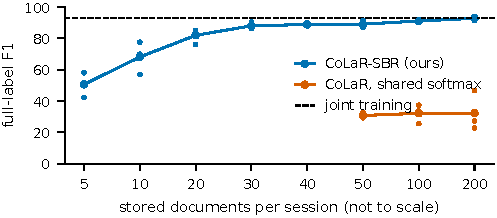
\includegraphics[width=0.6\textwidth]{paper/budget.pdf}
  \caption[Impact of the memory size]{\textbf{Impact of the memory size} on CIL-CORD:
  full-label F1 against stored documents per session (dots: runs; line: their mean; dashed:
  joint training).}
  \label{fig:budget}
\end{figure}

\begin{table}[!htbp]
  \centering
  \caption[Memory size on CIL-CORD: values]{\textbf{Memory size} on CIL-CORD (mean $\pm$
  s.d.; bold: the default size).}
  \label{tab:budget}
  % AUTO-GENERATED by scripts/rca/make_clean_tables.py -- do not edit.
\begin{tabular}{@{}lrcc@{}}
\toprule
Readout & Documents per session & Full-label F1 & AA \\
\midrule
Per-session (CoLaR-SBR) & 5 & $50.6{\pm}7.9$ & $59.9{\pm}3.6$ \\
 & 10 & $68.1{\pm}10.4$ & $73.8{\pm}3.4$ \\
 & 20 & $81.9{\pm}5.1$ & $84.0{\pm}2.3$ \\
 & 30 & $88.0{\pm}2.1$ & $86.0{\pm}2.8$ \\
 & 40 & $88.9{\pm}1.1$ & $87.6{\pm}1.8$ \\
 & \textbf{50} & $89.1{\pm}2.0$ & $88.4{\pm}2.6$ \\
 & 100 & $91.1{\pm}0.9$ & $90.1{\pm}1.0$ \\
 & 200 & $92.8{\pm}1.3$ & $92.7{\pm}1.0$ \\
\midrule
Shared softmax (CoLaR) & \textbf{50} & $30.7{\pm}1.5$ & $33.5{\pm}1.0$ \\
 & 100 & $32.1{\pm}6.0$ & $27.7{\pm}7.4$ \\
 & 200 & $32.2{\pm}12.7$ & $31.0{\pm}6.0$ \\
\bottomrule
\end{tabular}

\end{table}

\paragraph{Impact of the SVD rank.} The rank decides how faithfully a stored document is
kept (Table~\ref{tab:analysis}). As the results demonstrate, a smaller rank hurts our
method: at rank $64$, CoLaR-SBR falls to $\vSbrRankSixtyFourFull$ full-label F1 and becomes
unstable, and at rank $32$ it falls to $\vSbrRankThirtyTwoFull$, i.e.,
$\nSbrRankThirtyTwoDropMin$ to $\nSbrRankThirtyTwoDropMax$ points below rank $128$. This
indicates the importance of keeping the whole document faithfully. Thus, it is suggested
that a rank of $128$ ensures decent performance.

\paragraph{Impact of the injection layer.} The layer $k$ decides how many layers are
frozen and how many are trained on the stored documents. With $k=2$, $6$ or $8$, CoLaR-SBR
stays between $\nAnaLayerLo$ and $\nAnaLayerHi$ full-label F1, against $\vSbrFull$ with
$k=4$. Hence, our method is not sensitive to this setting, and we keep $k=4$.

\paragraph{Impact of the replayed documents per batch.} We replay two, four or eight
stored documents with each batch of two current documents. The results stay between
$\nAnaReplayLo$ and $\nAnaReplayHi$ full-label F1. Hence, our method is not sensitive to
this setting either, and we keep four replayed documents.

\begin{table}[!htbp]
  \centering
  \caption[Settings of CoLaR-SBR]{\textbf{Settings of CoLaR-SBR} on CIL-CORD: one setting
  changes at a time (bold: the default; mean $\pm$ s.d.).}
  \label{tab:analysis}
  % AUTO-GENERATED by scripts/rca/make_clean_tables.py -- do not edit.
\begin{tabular}{@{}lccc@{}}
\toprule
Setting & Value & Full-label F1 & AA \\
\midrule
SVD rank & 32 & $27.4{\pm}2.5$ & $33.1{\pm}2.5$ \\
 & 64 & $79.4{\pm}16.5$ & $81.4{\pm}12.9$ \\
 & \textbf{128} & $89.1{\pm}2.0$ & $88.4{\pm}2.6$ \\
\midrule
Injection layer $k$ & 2 & $88.7{\pm}1.1$ & $87.6{\pm}2.4$ \\
 & \textbf{4} & $89.1{\pm}2.0$ & $88.4{\pm}2.6$ \\
 & 6 & $90.6{\pm}1.8$ & $89.0{\pm}1.8$ \\
 & 8 & $88.1{\pm}2.0$ & $84.7{\pm}2.7$ \\
\midrule
Replayed documents per batch & 2 & $90.0{\pm}1.1$ & $89.3{\pm}1.9$ \\
 & \textbf{4} & $89.1{\pm}2.0$ & $88.4{\pm}2.6$ \\
 & 8 & $90.2{\pm}2.2$ & $89.0{\pm}2.8$ \\
\bottomrule
\end{tabular}

\end{table}

\section{Robustness}
\label{sec:c6-s6}
% SOURCE: session order, BROS + E2 encoders, patience
\todo{to be written}

\section{Memory and Computational Cost}
\label{sec:c6-s7}
% SOURCE: paper App. B memory analysis; E6 cost table
\todo{to be written}

\section{Beyond Documents: Image Classification}
\label{sec:c6-s8}
% SOURCE: paper App. F; E4
\todo{to be written}

\section{Qualitative and Error Analysis}
\label{sec:c6-s9}
% SOURCE: receipt figure, per-class results, where the owner block errs
\todo{to be written}

\section{Discussion}
\label{sec:c6-s10}
% SOURCE: answers to RQ1-RQ4; relation to prior work
\todo{to be written}

